\documentclass[11pt,a4paper]{article}

\usepackage{geometry}
\geometry{margin=2.5cm}
\usepackage{graphicx}
\usepackage{xurl}
\usepackage{doi}
\usepackage{natbib}
\usepackage{hyperref}
\hypersetup{colorlinks=true, urlcolor=black, linkcolor=black, citecolor=black}

\begin{document}

\renewcommand{\thefigure}{S\arabic{figure}}
\setcounter{figure}{0}

% \section*{Supplementary Material}


\begin{figure}[!ht]
\centering
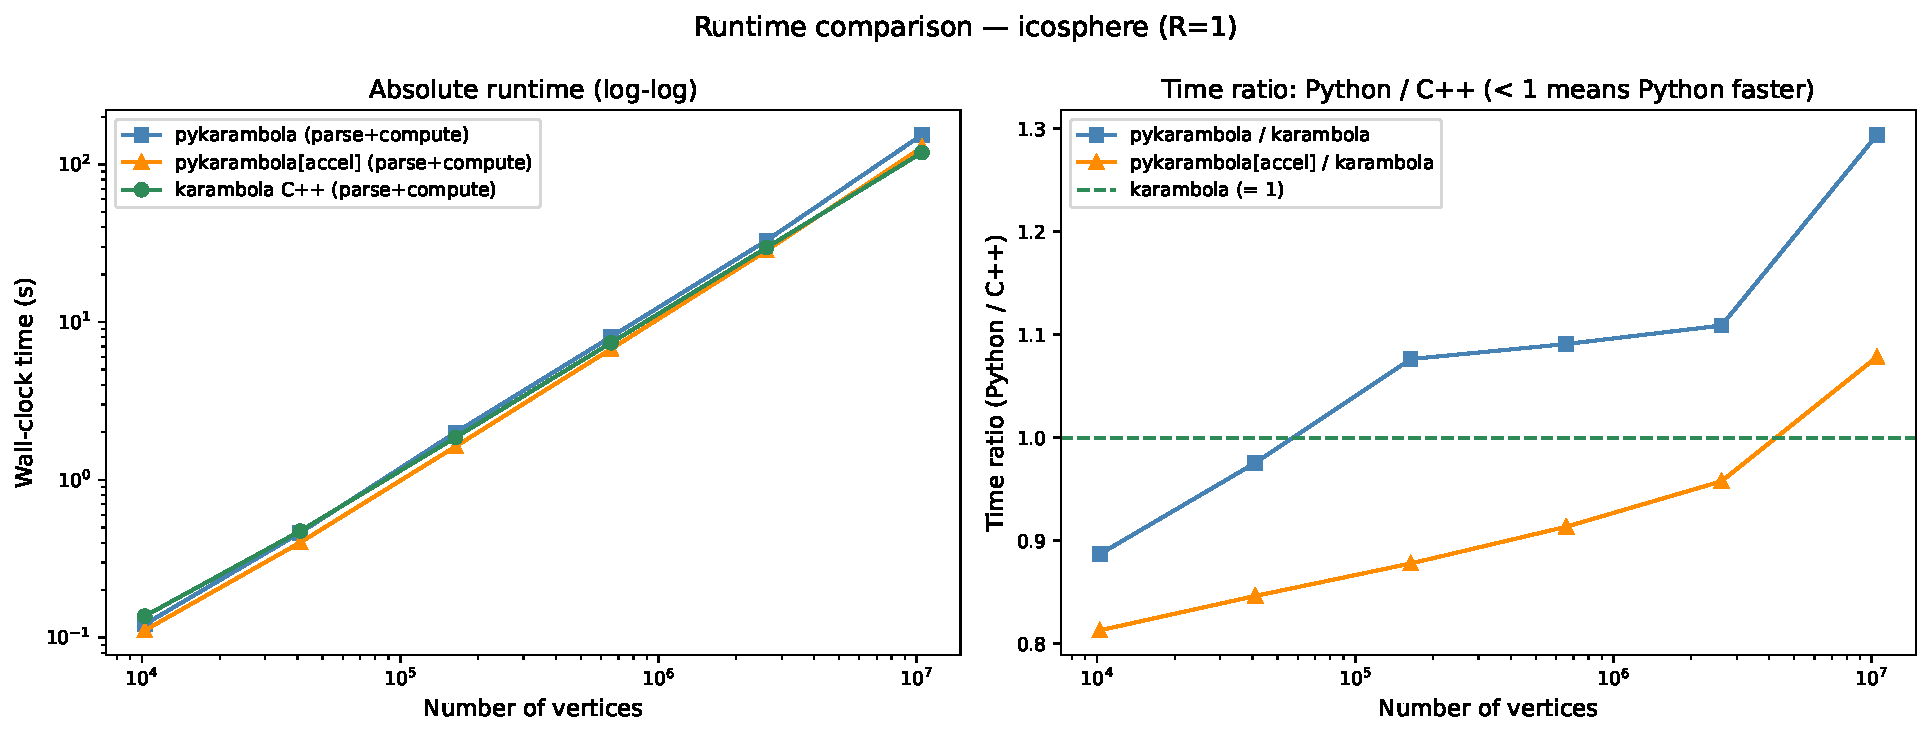
\includegraphics[width=\textwidth]{notebooks/results/timing_comparison_option_a.pdf}
\caption{Runtime benchmark on synthetic icospheres (subdivision levels 5--10; 10{,}242--10{,}485{,}762 vertices).
\textbf{Left}: absolute wall-clock time (log-log scale) for end-to-end execution (mesh parse + Minkowski tensor compute) for C++ karambola (green), pykarambola pure-Python (blue), and pykarambola Cython-accelerated (orange).
\textbf{Right}: speedup ratio (karambola time / pykarambola time); values above the dashed line ($= 1$) indicate pykarambola is faster.
\textit{Alt text: two-panel figure. Left panel: log-log line plot of wall-clock time versus mesh vertex count for three implementations (karambola, pure-Python, Cython); all three scale similarly with the Cython build closest to or faster than karambola. Right panel: speedup ratio versus vertex count; pure-Python line sits below 1 at small sizes and approaches 1 at large sizes; Cython line stays at or above 1 across the full range.}}
\label{fig:runtime}
\end{figure}

%
\begin{figure}[!ht]
\centering
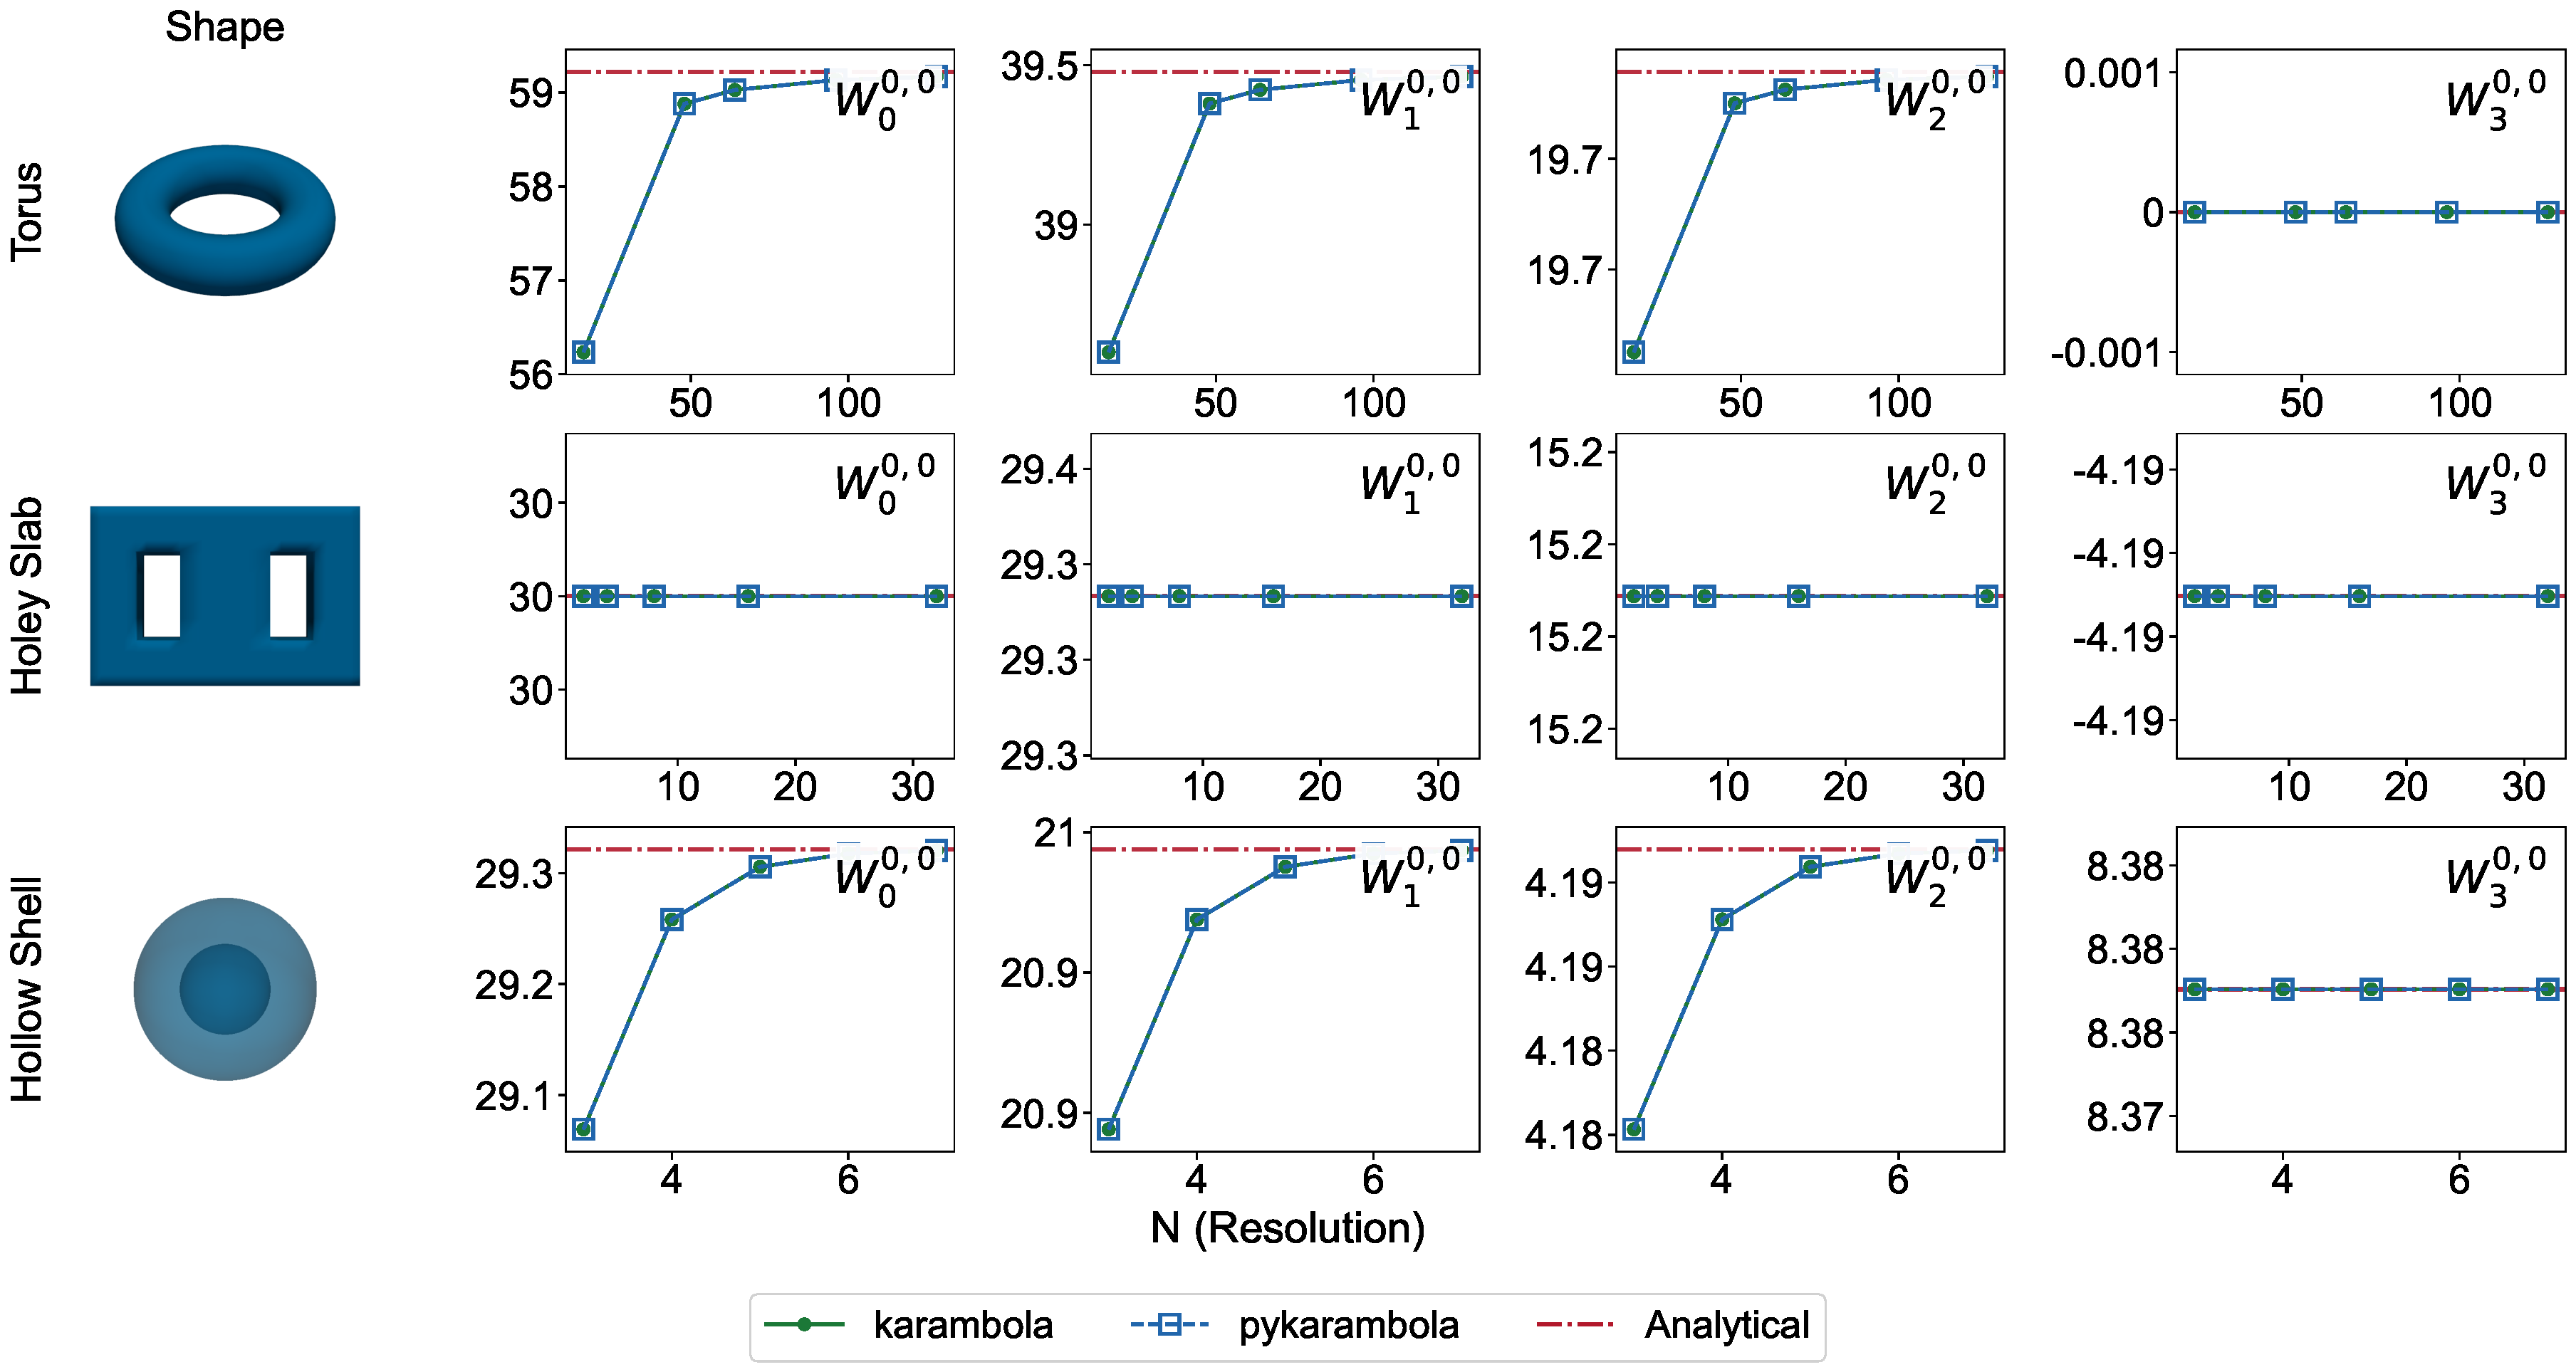
\includegraphics[width=0.95\textwidth]{notebooks/results/topology_convergence.pdf}
\caption{%
  Resolution convergence of \texttt{pykarambola} and C++ \texttt{karambola} toward analytical Minkowski scalar values on three synthetic meshes of known topology.
  Each plot panel shows one scalar Minkowski functional against mesh resolution~$n$ for karambola (green, solid, filled circles), pykarambola (blue, dashed, open squares), and the analytical value (red dash-dot line).
  The leftmost column (\emph{Shape}) shows a representative 3D rendering of each mesh.
  Rows correspond to shapes: torus ($\chi = 0$, genus~1), holey slab (rectangular slab with two rectangular through-holes, $\chi = -2$, genus~2), and hollow shell (two nested icospheres, $\chi = +4$, two components).
  The four plot columns correspond to the four scalar Minkowski functionals: volume $W_0^{0,0}$, surface area $W_1^{0,0}$, integrated mean curvature $W_2^{0,0}$, and the topological term $W_3^{0,0}$ ($\propto \chi$).
  Both implementations converge toward the analytical values with increasing resolution and agree with each other to near floating-point precision at every resolution; $W_3^{0,0}$ is a topological invariant and is reproduced exactly at all resolutions.
  Each shape was evaluated at five mesh resolutions.
  \textit{Alt text: a grid of panels with three rows (torus, holey slab, hollow shell). The leftmost column shows a 3D rendering of each shape; the remaining four columns are line plots of the volume, surface area, integrated mean curvature, and topological scalar Minkowski functionals against mesh resolution. In each line plot a green solid curve (karambola) and a blue dashed curve (pykarambola) nearly coincide and approach a red dash-dot horizontal line marking the analytical value as resolution increases, with residual differences at the level of floating-point precision. The topological-term panels are essentially flat on the analytical value at all resolutions.}
}
\label{fig:topology}
\end{figure}


\begin{figure}[!ht]
\centering
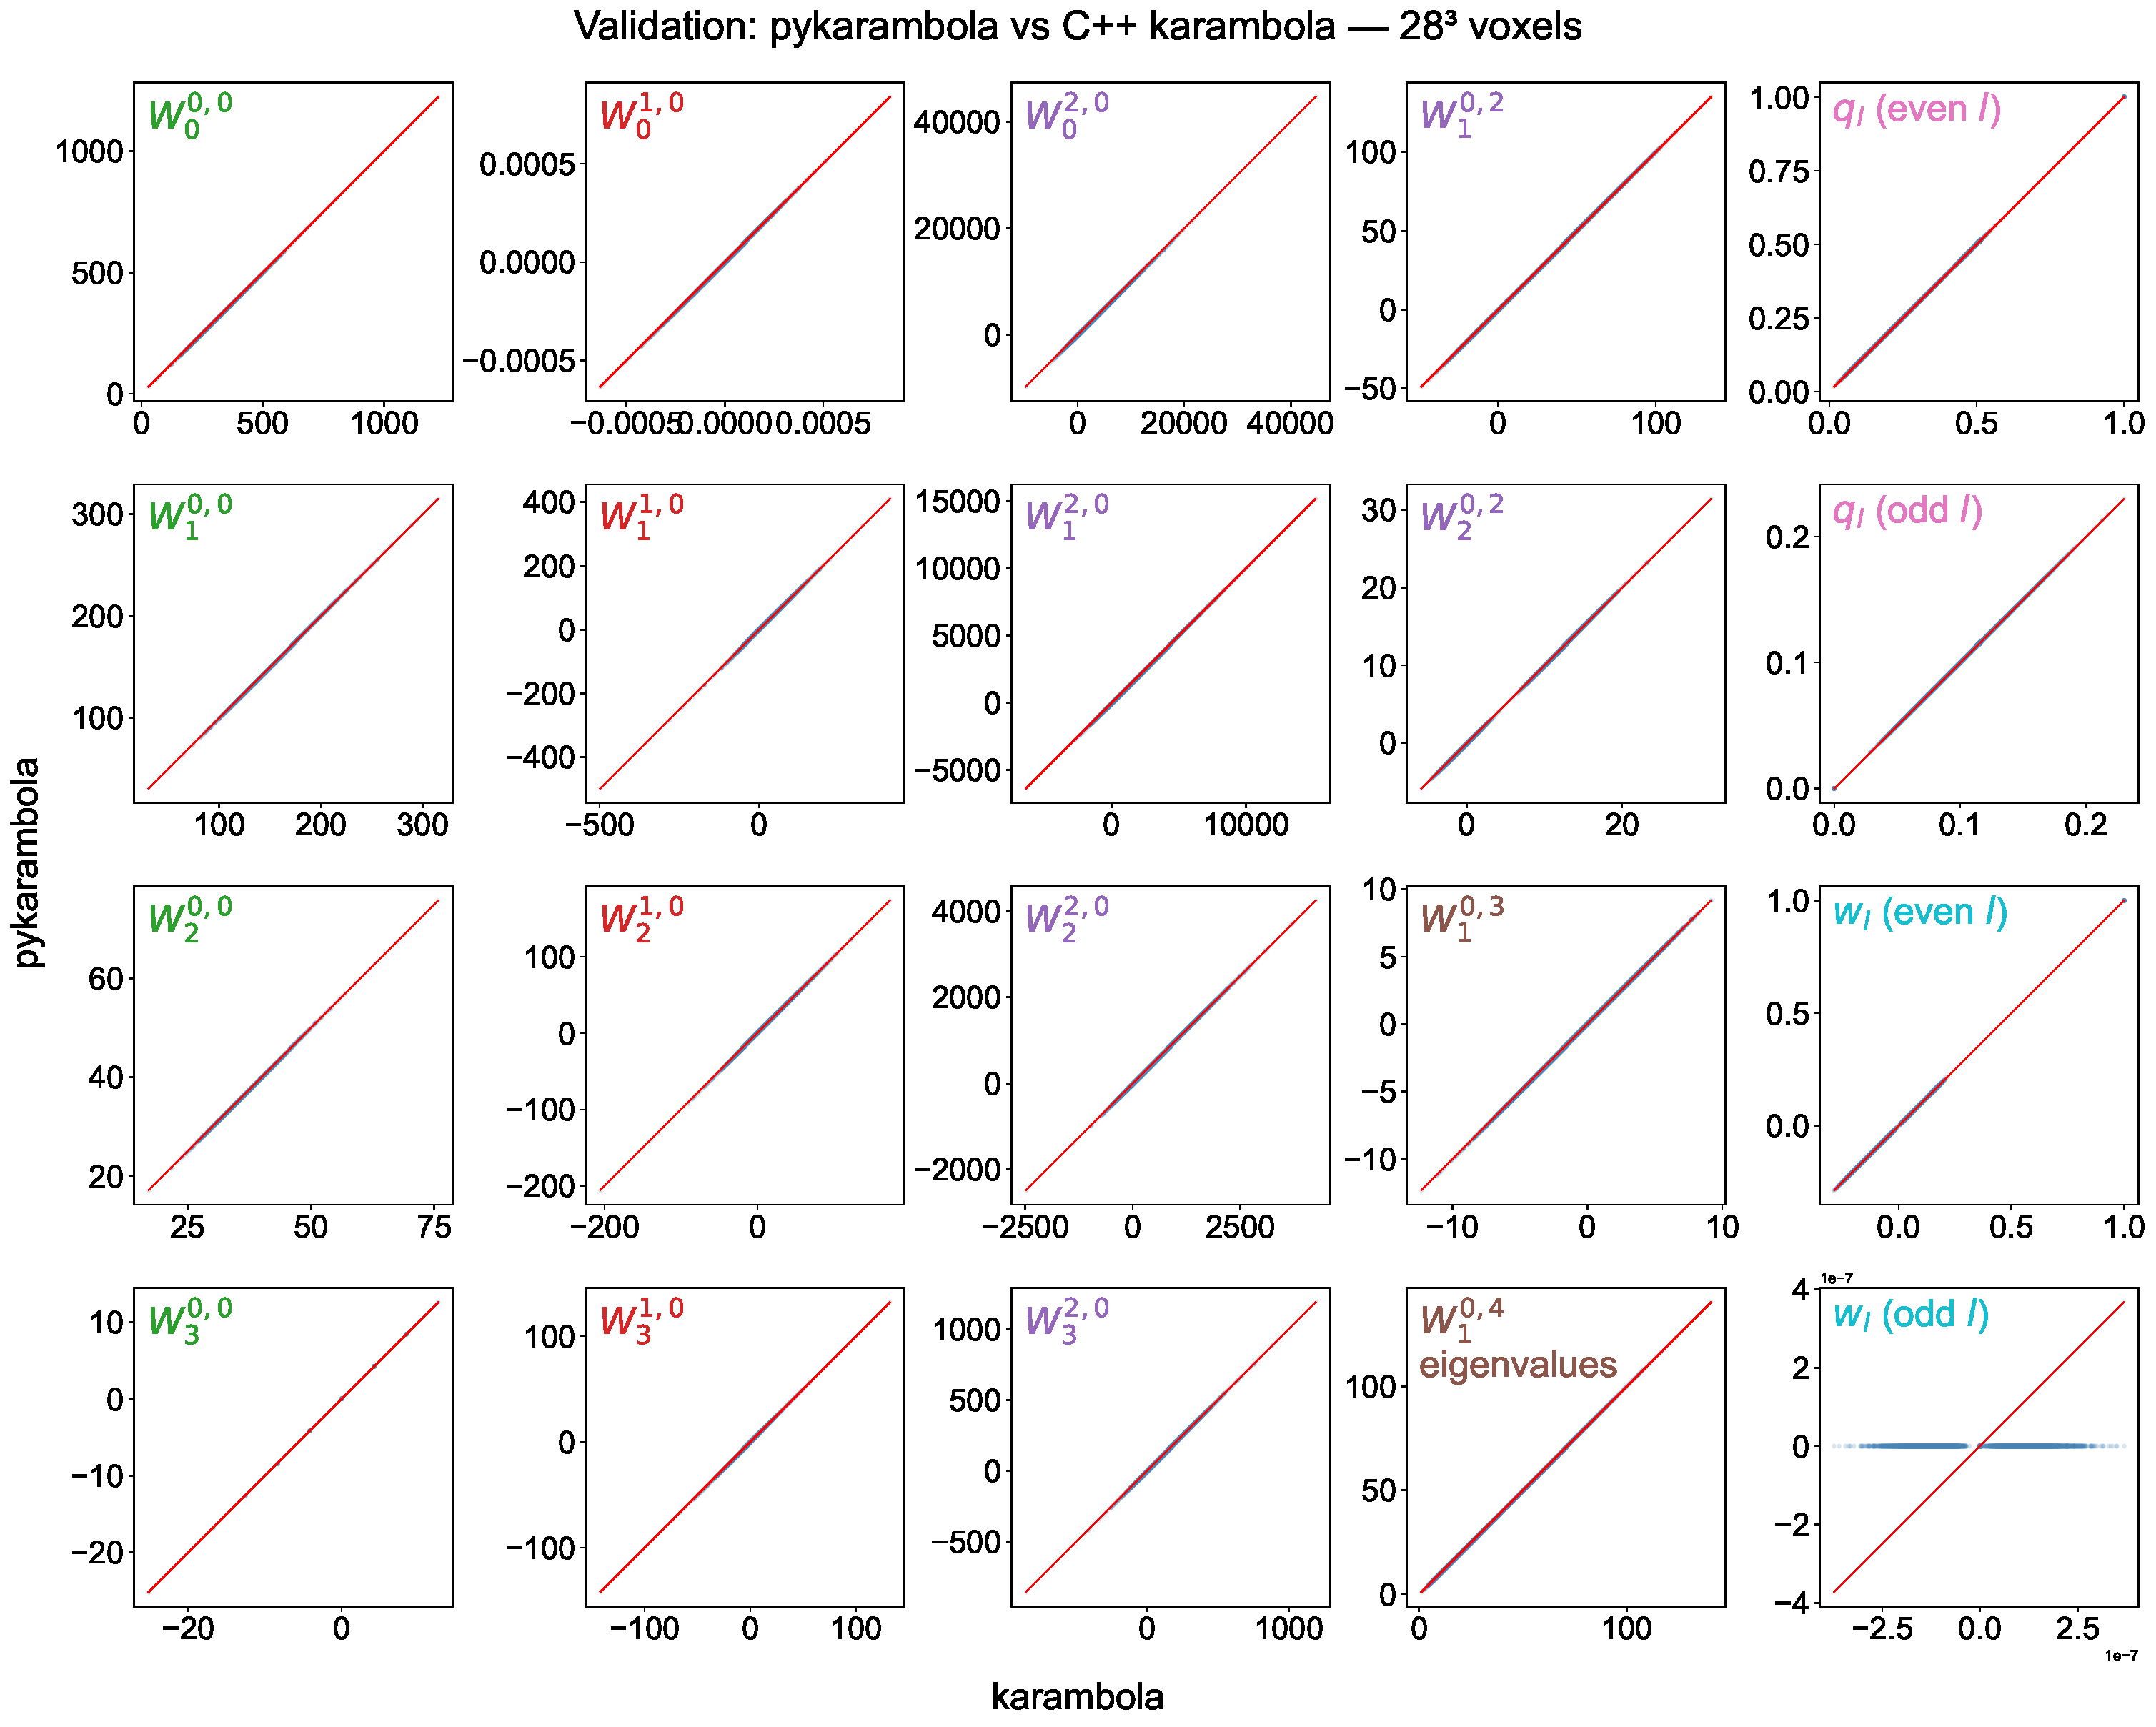
\includegraphics[width=0.95\textwidth]{notebooks/results/scatter_accuracy_paper.pdf}
\caption{Numerical accuracy of pykarambola relative to C++ karambola.
Each panel shows a scatter plot of values from identical analyses run in C++
(karambola, $x$-axis) and Python (pykarambola, $y$-axis) on
the AdrenalMNIST3D dataset (1{,}584 meshes, $28^3$ voxel resolution).
Columns correspond to feature groups: scalars ($W_\nu^{0,0}$),
vectors ($W_\nu^{1,0}$), rank-2 tensors ($W_\nu^{2,0}$, $W_\nu^{0,2}$),
and higher-rank quantities ($W_1^{0,3}$, $W_1^{0,4}$ eigenvalues, and spherical
Minkowski summary quantities $q_l$ and $w_l$).
Panel labels are shown in the top-left corner of each panel, colored by feature group.
The red diagonal indicates perfect agreement; all points fall on this line except
odd-$l$ \texttt{msm\_wl}, which pykarambola returns as exactly zero
while karambola produces small spurious residuals (see text).
Equivalent agreement is observed at $64^3$ resolution (Supplementary Figure~S4).
\textit{Alt text: a grid of scatter plots with four columns (scalars, vectors, rank-2 tensors, higher-rank and MSM quantities) and multiple rows, one per feature. The $x$-axis shows C++ karambola values and the $y$-axis shows pykarambola values; a red diagonal marks perfect agreement. All scalar and tensor panels show points tightly on the diagonal; odd-$l$ msm\_wl panels show pykarambola at exactly zero while karambola has small non-zero residuals.}}
\label{fig:accuracy}
\end{figure}

\begin{figure}[!ht]
\centering
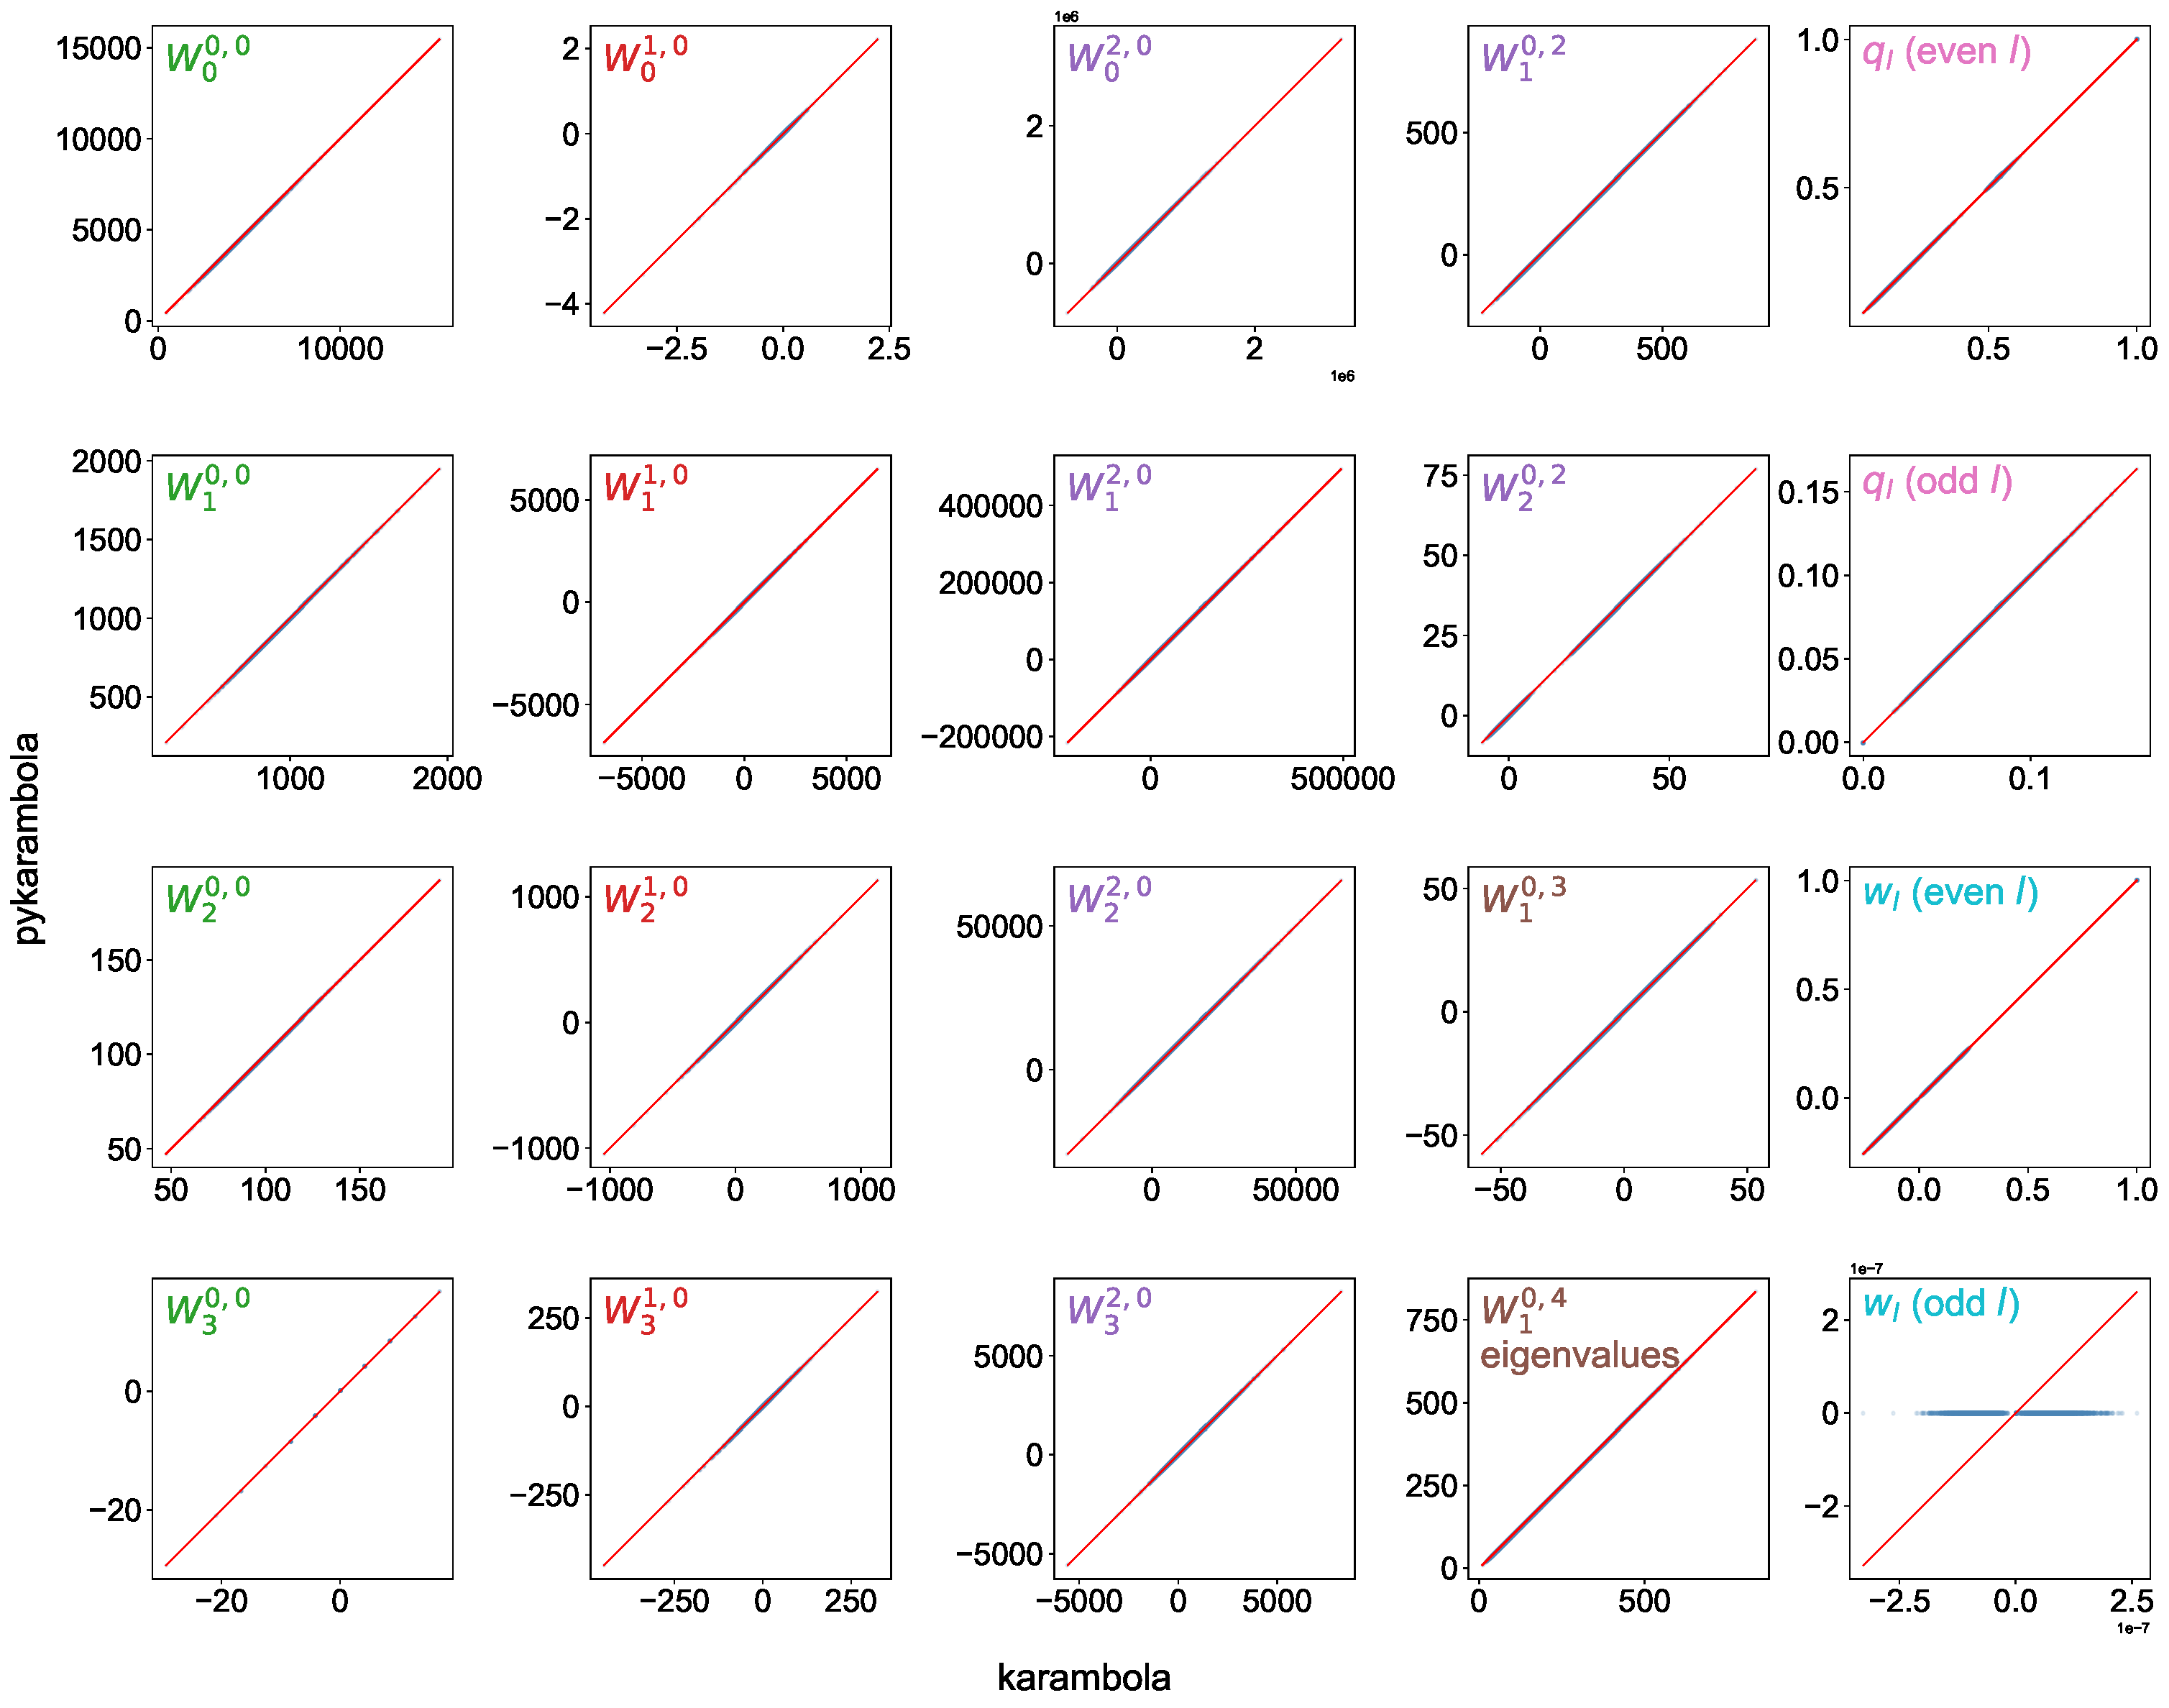
\includegraphics[width=0.95\textwidth]{notebooks/results/scatter_accuracy_paper_supplementary.pdf}
\caption{Numerical accuracy of pykarambola relative to C++ karambola at $64^3$ voxel resolution.
All panels and groupings are identical to Supplementary Figure~S3.
\textit{Alt text: same layout as Supplementary Figure~S3 at $64^3$ voxel resolution; all points lie on the red diagonal indicating perfect agreement between the two implementations.}}
\label{fig:accuracy_supp}
\end{figure}

%
\begin{figure}[!ht]
\centering
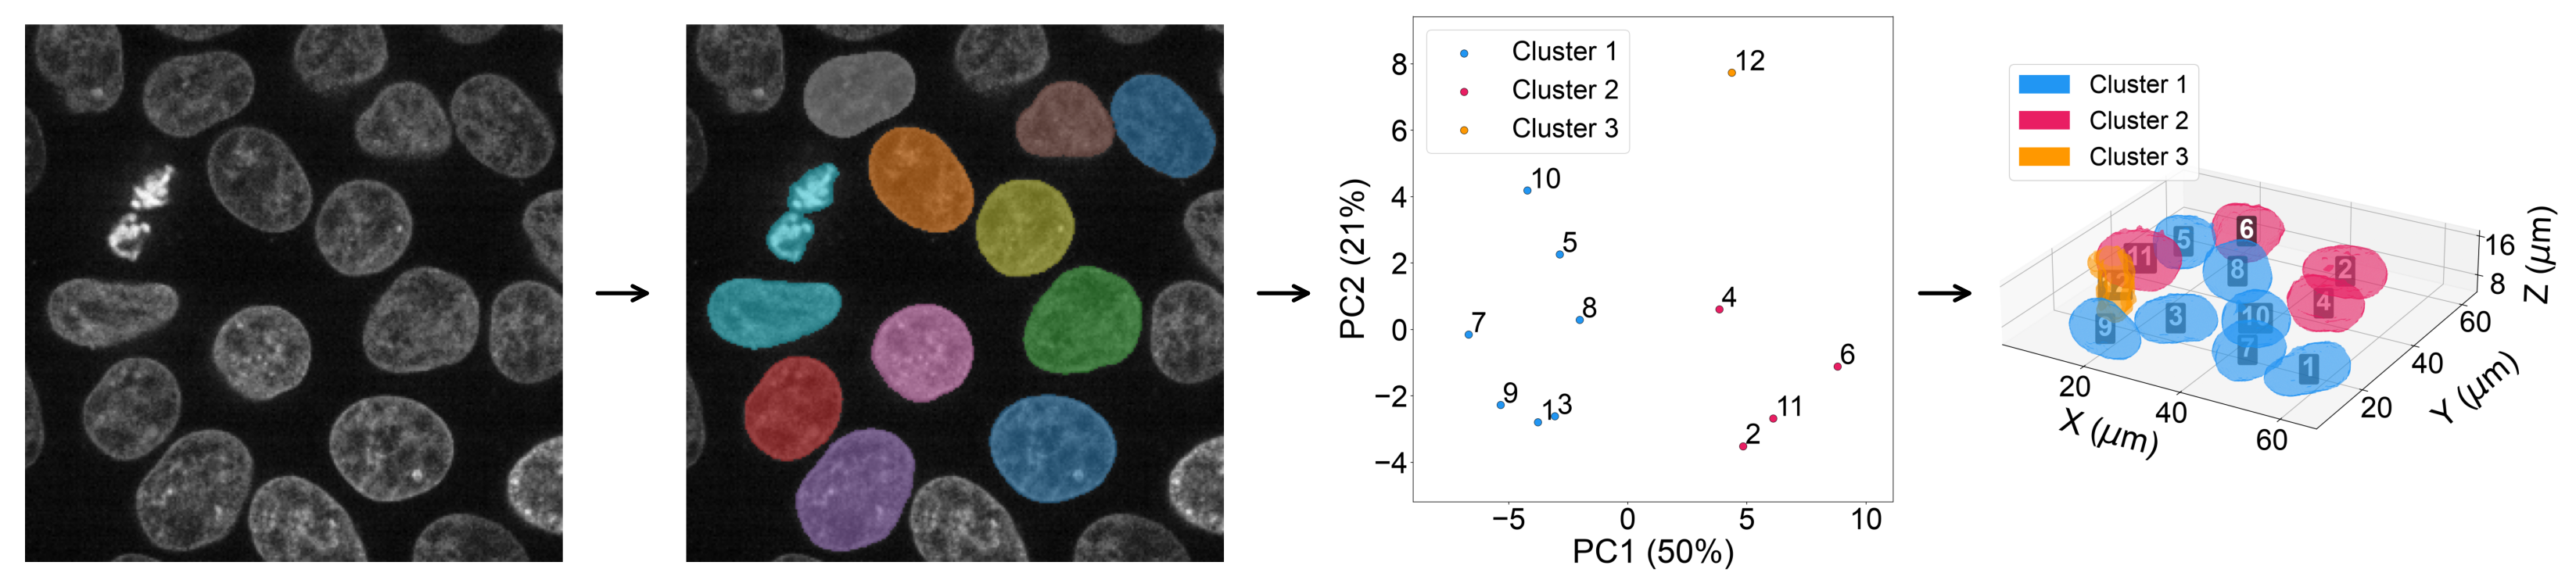
\includegraphics[width=\textwidth]{../assets/demo_pipeline.png}
\caption{%
  End-to-end segmentation-to-morphometry pipeline applied to 3D confocal nuclei (\texttt{skimage.data.cells3d}~\citep{vanderwalt2014scikit}).
  From left to right: (i)~raw fluorescence stack (nuclei channel), mid-Z slice shown; (ii)~integer label image produced by scikit-image watershed segmentation, each colour representing one of 12 individually resolved non-border-touching nuclei; (iii)~PCA projection of the rotationally invariant subset of tensor outputs (Minkowski scalars, $\beta$, eigenvalues, trace, and MSM $q_l/w_l$; 56 features per nucleus) computed in a single \texttt{minkowski\_tensors\_from\_label\_image} call, points coloured by hierarchical agglomerative cluster assignment; (iv)~3D surface meshes of all nuclei coloured by the same cluster assignment; the spatially isolated nucleus (orange) is the mitotic cell (lower $\beta$, larger volume).
  The complete pipeline is provided in \texttt{examples/segmentation\_workflow.ipynb}.
  \textit{Alt text: four-panel horizontal figure connected by arrows showing a left-to-right pipeline. First panel: grey-scale confocal mid-Z slice. Second panel: colour-coded integer segmentation overlay. Third panel: 2D PCA scatter plot with three coloured clusters. Fourth panel: 3D mesh render with nuclei coloured by cluster; one orange nucleus is spatially isolated.}
}
\label{fig:workflow}
\end{figure}


\begin{figure}[!ht]
\centering
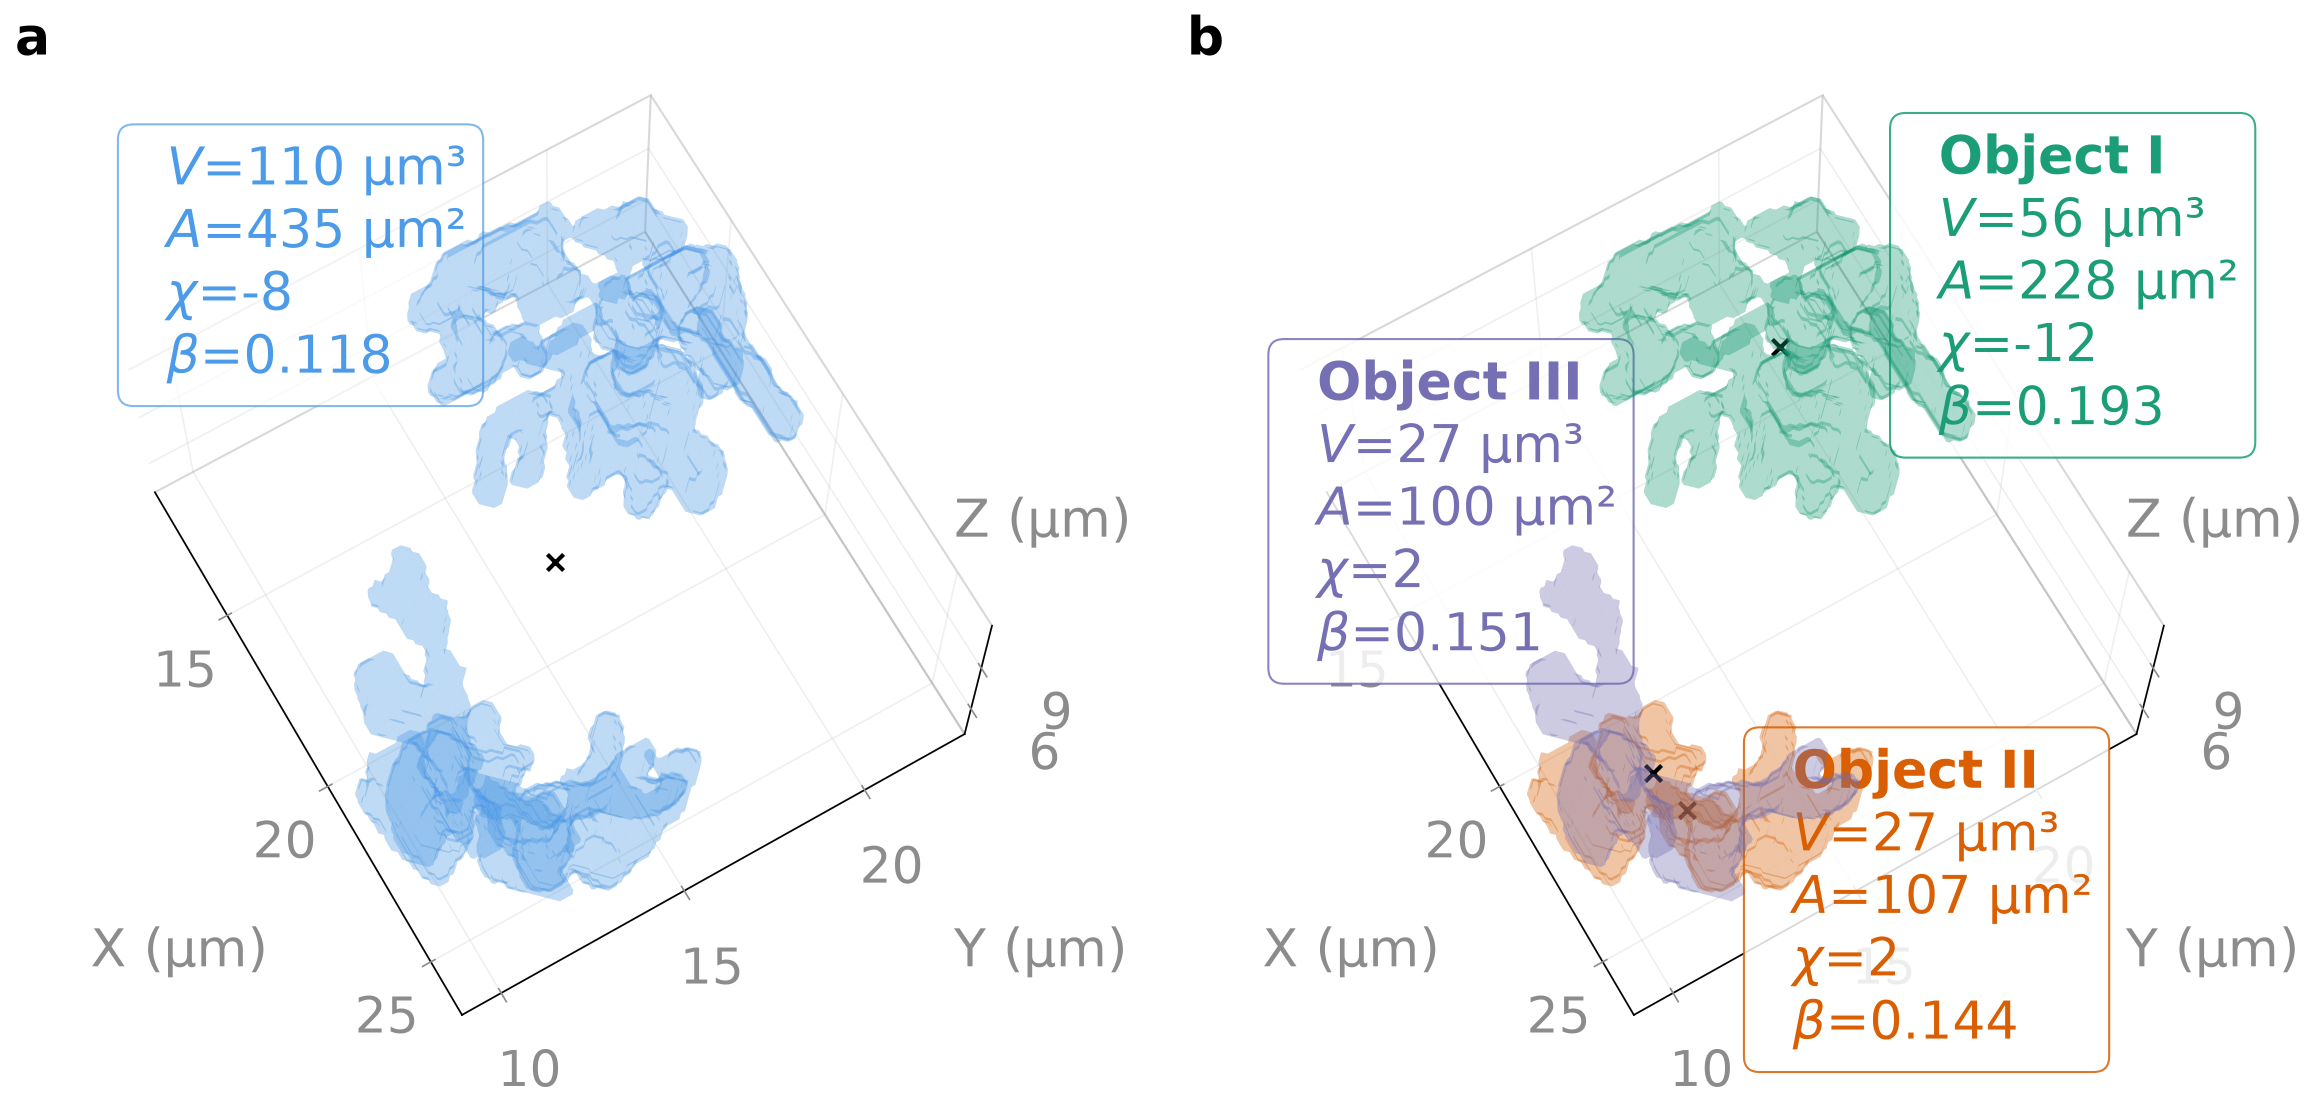
\includegraphics[width=\linewidth]{../assets/figure21.png}
\caption{%
  Label-image API applied to the DNA channel of a 3D fluorescence microscopy segmentation
  of a hiPSC in anaphase/telophase (Allen Cell Collection~\citep{viana2023integrated};
  isotropic voxel size 0.108\,$\mu$m).
  Per-object Minkowski tensors report volume~($V$), surface area~($A$),
  Euler characteristic~($\chi$), and anisotropy index~($\beta$),
  with object centroids marked~($\times$).
  (\textbf{a}) The entire DNA channel assigned as a single label;
  one tensor set describes the aggregate of all three DNA objects ($V=110$\,$\mu$m$^3$, $A=435$\,$\mu$m$^2$, $\chi=-8$, $\beta=0.118$).
  (\textbf{b}) The binary DNA mask passed with \texttt{autolabel=True};
  pykarambola detects three connected components internally and returns
  three independent tensor sets, one per DNA object (Object~I: $\chi=-12$; Objects~II--III: $\chi=2$ each).
  Objects~2 and~3 occupy non-overlapping axial ranges (Z slices 40--72 and 78--110,
  respectively) and are likely segments of the same daughter chromosomal mass.
  \textit{Alt text: two 3D mesh renders of chromosomal DNA. Left panel (a): a single blue semi-transparent mesh of the aggregate chromatin mass, annotated with V, A, chi, and beta values. Right panel (b): three separately coloured meshes for individual DNA objects, each annotated with its own V, A, chi, and beta values and a centroid cross marker.}
}
\label{fig:labelimage}
\end{figure}

%
\begin{figure}[!ht]
\centering
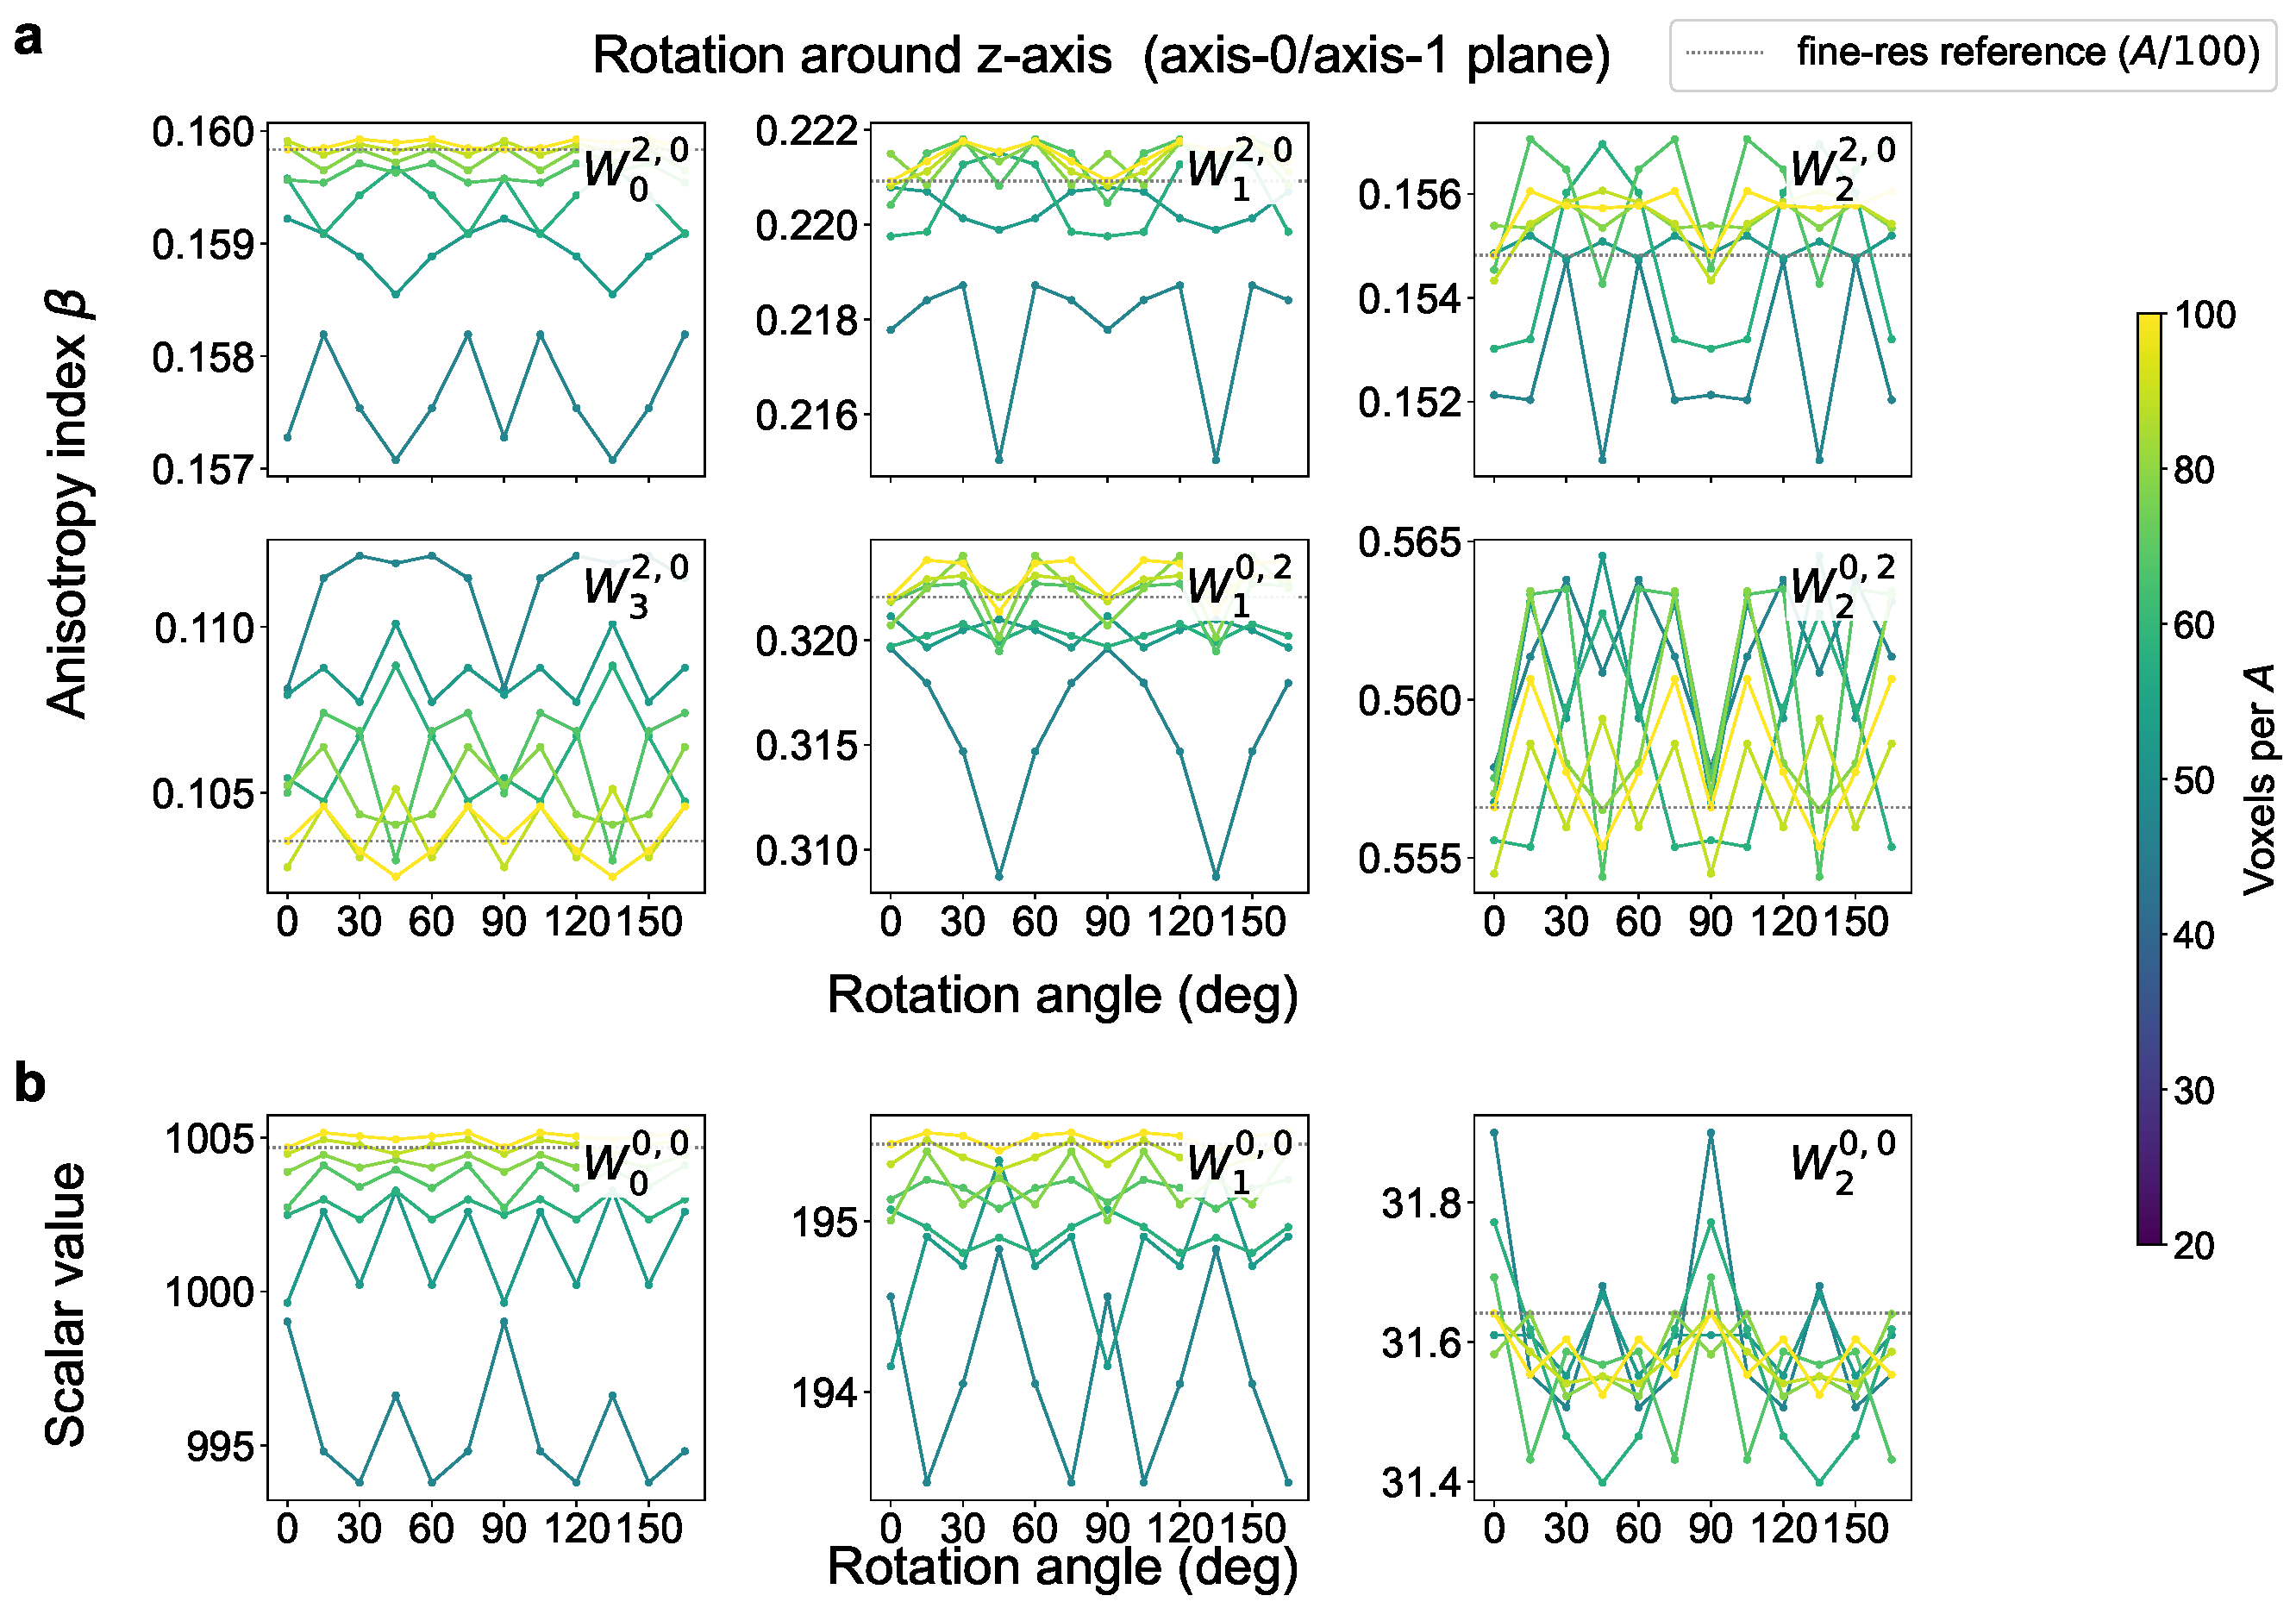
\includegraphics[width=0.95\textwidth]{notebooks/results/orientation_bias_beta_combined_rot_z.pdf}
\caption{%
  Orientation dependence of Minkowski measures under grid rotation.
  A synthetic triaxial ellipsoid (semi-axes $A=10$, $B=6$, $C=4$, in
arbitrary distance units) was rotated about the $z$-axis through 12 orientations ($0^\circ$--$165^\circ$ in $15^\circ$ steps) at seven grid resolutions (20--100 voxels per semi-axis~$A$; colour scale).
Each curve traces one measure against rotation angle at fixed resolution; the periodic variation with angle is the orientation-induced discretisation artefact, and its amplitude decreases with increasing resolution as the curves converge toward the dotted reference.
The dotted black line is the fine-resolution reference, evaluated at the finest grid (100 voxels per~$A$) at $0^\circ$ orientation.
(\textbf{a})~Anisotropy index $\beta = \lambda_\mathrm{min}/\lambda_\mathrm{max}$ (ratio of smallest to largest tensor eigenvalue) for the six rank-2 Minkowski tensors $W_0^{2,0}$, $W_1^{2,0}$, $W_2^{2,0}$, $W_3^{2,0}$, $W_1^{0,2}$, $W_2^{0,2}$.
(\textbf{b})~Value of the three scalar Minkowski functionals $W_0^{0,0}$ (volume), $W_1^{0,0}$ (surface area), and $W_2^{0,0}$ (integrated mean curvature); the topological functional $W_3^{0,0}$ is omitted as it is an integer invariant unaffected by orientation and resolution.
\textit{Alt text: a nine-panel figure, six panels in (a) and three in (b), each plotting a morphometric measure against rotation angle from 0 to 165 degrees, with one coloured line per grid resolution from 20 (dark) to 100 (light) voxels per semi-axis.
All curves oscillate periodically with angle; the oscillation amplitude shrinks and the curves approach a dotted black reference line as resolution increases.}
}
\label{fig:orientation_bias}
\end{figure}


% Issues #168 and #170: resolved — see topology_validation.ipynb and orientation_bias.ipynb.
% Issue #164: fig:workflow moved to supplementary.

\clearpage
\bibliographystyle{plainnat}
\bibliography{references}

\end{document}
